\chapter{RISC-V} % Main chapter title
\label{RISC-V} % For referencing the chapter elsewhere, use \ref{Chapter1} 

\section{Einleitung}
\emph{RISC-V} ist eine offene Befehlssatzarchitektur, die 2010 von Entwicklern an der University of California, Berkeley vorgestellt wurde. Sie basiert auf der RISC (reduced instruction set computing) Design\textit{philosophie} basiert. 

???Falsch: In Abgrenzung zu CISC (complex instruction set computing) sind RISC Befehlssätze leichtgewichtiger, d. h. es werden in der Regel weniger Maschineninstruktionen definiert. ??Vor-Nachteile?

Ein wichtiger Vorteil von RISC-Architekturen, insbesondere im Hinblick auf das vorliegende Projekt, liegt in der einfachen Implementierung. 

Beim Entwurf wurde besonderer Wert auf eine leichtgewichtige Architektur, aber auch Performance und Energiesparsamkeit gelegt.

Eine Befehlssatzarchitektur definiert den Befehlssatz einer CPU. Sie spezifiziert u. a., welche Maschinenbefehle eine CPU verarbeiten können muss, was genau ihre Ausführung bewirkt wie sie mit dem Speicher interagiert und definiert und wie definiert CPU eigene Speicherbänke (Register). Sie stellt damit die Schnittstelle zwischen der Hardware und Software einer Maschine dar. Mithilfe einer solchen einheitlichen Schnittstelle kann Software ohne Kenntnis der zugrunde liegenden Hardware Software für eine Maschine programmieren.

Von der Befehlssatzarchitektur abzugrenzen ist die Mikroarchitektur, die die Implementierung des Befehlssatzes auf einem Chip bestimmt.

Für dieses Projekt wurde der RISC-V (Link?!) Befehlssatz übernommen, und eine eigene Hardware-Implementierung, die die Befehlssatzspezifikation von RISC-V erfüllt, entwickelt.


%----------------------------------------------------------------------------------------
\section{RISC-V Varianten und verwendetes Instruktionssubset}

\paragraph{Wortbreite.} Für RISC-V Architekturen sind die Wortbreiten $32, 64$ und $128$bit vorgesehen.

\paragraph{Erweiterungen.} Die RISC-V Architektur ist darauf ausgelegt, flexibel erweiterbar zu sein. Die Spezifikation definiert daher mehrere Teilmengen des allgemeinen Befehlssatzes. \citep[p. 4]{RISC}

Um die RISC-V Anforderungen zu erfüllen, muss eine Implementierung zumindest die Basisinstruktionen zur Integerverarbeitung umsetzen (Bezeichnung nach RISC-V Konvention: \textit{I})

Die allgemeine als \textit{General Purpose} bezeichnete Architektur enthält neben diesem Mindeststandard auch Befehle für Gleitkommaarithmetik (F) mit Double(D) oder Quad-Präzision (Q), für die Handhabung verschiedener Privilegierungen (P), atomare Befehle für die Verwaltung von Nebenläufigkeit (A) und seit der neusten Version 2.1 auch für Bitmanipulation (B), Vectoroperationen (V) und einigen mehr.

\paragraph{Verwendetes Subset.} In diesem Projekt wurde sich allerdings darauf beschränkt, eine einfache integerverarbeitende Mikroarchitektur umzusetzen. Als Wortbreite wurden 32bit gewählt. Die Bezeichnung des verwendeten Subsets lautet daher nach RISC-V Konventionen \textit{RV32I}.
%----------------------------------------------------------------------------------------

%----------------------------------------------------------------------------------------
\section{RV32I}
Das verwendete Subset besteht aus $47$ verschiedenen Maschineninstruktionen.

\begin{figure} [ht]
  \centering
  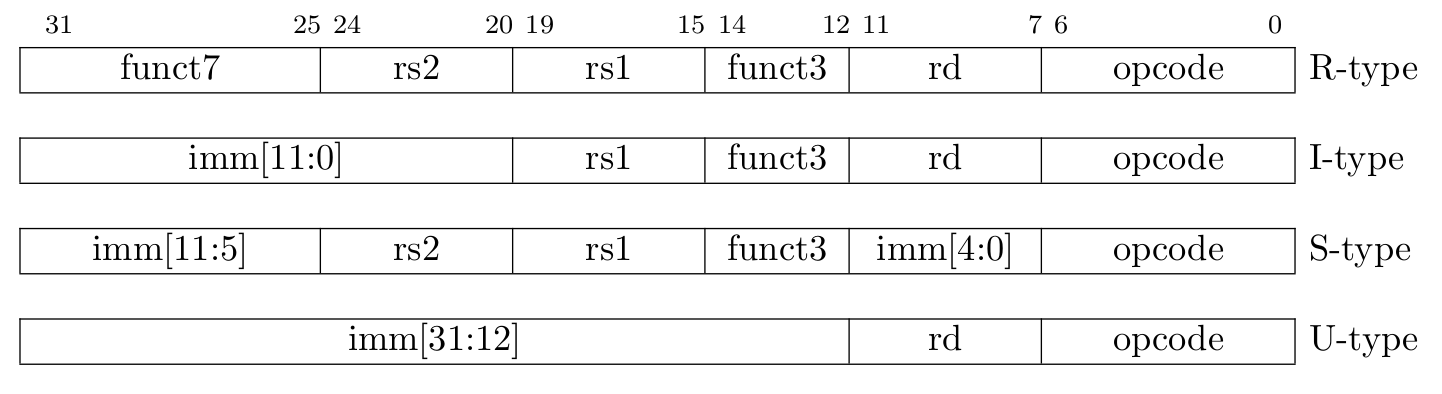
\includegraphics[width=0.95\textwidth]{Figures/instruction_formats}
  \caption{Instruktionsformate. Quelle: \citep[p. 11]{RISC}}
  \label{fig:instr_types}
\end{figure}

\subsection{Register}
???

\subsection{Instruktionsformate}
RV32I kennt vier verschiedene Formate, in denen Maschinen instruktionen enkodiert sein können: \textit{R-type}, \textit{I-Type}, \textit{S-type} und \textit{U-type} - Befehle.

%----------------------------------------------------------------------------------------

%----------------------------------------------------------------------------------------
\section{Architektur}
- branch delay slots?
\subsection{Speicherarchitektur}
RISC-V ist als \textit{load-store}-Architektur entworfen. Arithmetische und logische Instruktionen greifen daher nicht auf den Speicher zu, stattdessen werden alle Operatoren vorher in der Registerbank abgelegt. Rechenergebnisse werden ebenfalls in Registern gespeichert. Speicherzugriffe werden ausschließlich mit \textit{load} bzw. \textit{store}-Befehlen realisiert.

\subsection{Register}
Die RISC-V Spezifikation definiert 31 Integer Register 1 - 31. Zusätzlich existiert ein \textit{zero}-Register, das eine konstante 0 beinhaltet. Andere Register (Floating Point) können an dieser Stelle vernachlässigt werden, da sich die umgesetzte CPU auf Integerverarbeitung beschränkt.
%----------------------------------------------------------------------------------------

%----------------------------------------------------------------------------------------
\section{Maschinenbefehle}
RISC-V Maschinenbefehle haben eine fixe Länge, die der Wortlänge der Architektur entspricht?
\paragraph{Branches.} Branches blabla ed diam nonumy eirmod tempor invidunt ut labore et dolore magna aliquyam erat, sed diam voluptua. At vero eos et accusam et justo duo dolores et ea rebum. Stet clita kasd gubergren, no sea takimata sanctus est Lorem ipsum dolor sit amet.
\subsection{B}
%----------------------------------------------------------------------------------------